

\begin{table}[t!]
\centering
\footnotesize
\caption{\textbf{Total research articles processed for creating priority pathogen SLRs.} \textbf{PERG} indicates the total article count retrieved from \texttt{epireview} (R package) after deduplication; \textbf{\name{}} indicates articles downloaded after \name{}'s Article Search and Retrieval stage; \textbf{Matched} indicates their intersection. The coloured symbols represent the progress of PERG's SLRs per priority-pathogen: published \published{}, conducting data extraction \extractionphase{}, and yet to begin screening \notstarted{}, as of March 2026.}
\setlength{\tabcolsep}{3pt}
\renewcommand{\arraystretch}{1.1}
\label{tab:article_count_summary_ours_pergs}
\begin{tabular}{lrrr}
\toprule
\textbf{Pathogen} & \textbf{PERG\textsuperscript{*}} & \textbf{\name{}} & \textbf{Matched} \\
\midrule
\published{} Marburg virus & 2,593 & 6,501 & 762 (29.4\%) \\
\published{} Ebola virus & 11,605 & 23,226 & 3,938 (33.9\%) \\
\published{} Lassa fever & 2,131 & 6,514 & 647 (30.4\%) \\
\published{} SARS-CoV-1 & 12,280 & 7,540 & 1,967 (16.0\%) \\
\published{} Zika virus & 10,510 & 3,103 & 2,128 (20.2\%) \\
\extractionphase{} MERS-CoV & 19,656 & 23,204 & 5,675 (28.9\%) \\
\extractionphase{} Nipah virus & 1,458 & 5,103 & 664 (45.5\%) \\
\notstarted{} Rift Valley fever virus & -- & 6,810 & -- \\
\notstarted{}  CCHF virus & -- & 3,478 & -- \\
\midrule
\textbf{Total}$^{\dagger}$ & 60,233 & 75,191 & 15,781 (26.2\%) \\
\bottomrule
\end{tabular}
% \vspace{0.5pt}
\par{\scriptsize
\textsuperscript{*}Articles post deduplication and empty abstract removal. \\
$^{\dagger}$Excludes Rift Valley fever virus and CCHF virus article counts.}
\end{table}



\section{Methods}

\subsection{Data}
\label{sec:methods_data}
For evaluation against ground truth, we used SLRs from the Pathogen Epidemiology Review Group (PERG) and their corresponding data made available through the \texttt{epireview} and \texttt{priority-pathogen} R packages \cite{naidooEpireviewToolsUpdate2025, nashPrioritypathogens2026}. PERG is conducting SLRs for nine ``priority pathogens'' identified by the WHO as having high epidemic or pandemic potential \cite{worldhealthorganizationPathogensPrioritizationScientific2024}. The group has published five peer-reviewed SLRs \cite{cuomo-dannenburgMarburgVirusDisease2024, doohanLassaFeverOutbreaks2024, nashEbolaVirusDisease2024, morgensternSevereAcuteRespiratory2025,mccain2026systematic} and two more (MERS and Nipah) are in the data extraction phase. For these seven pathogens, approximately $26.2\%$ of the articles considered by PERG were available under open-access licensing through the bibliographic databases we queried (\Cref{tab:article_count_summary_ours_pergs}). We evaluated each \name{} stage with all pathogen data available, meaning the first seven are evaluated for screening, and four (Ebola, Lassa, SARS, and Zika) are evaluated for data extraction. After correspondence with PERG, we chose to exclude Marburg due to inconsistencies in data format, and MERS and Nipah because PERG's extraction phase is still in progress.



\subsection{Models}
% We implemented \name{} with OpenAI's open-weight \texttt{gpt-oss-120b} model \cite{openai2025gptoss120bgptoss20bmodel}. Note that the pipeline is extensible to any model accessed via API. \texttt{gpt-oss-120b} has a context length of 131,072 tokens; articles require approximately 32,000 input tokens, and the remaining $\sim$100,000 are frequently fully used for prompt input, reasoning and tool calling. We host the model with \texttt{vllm} \cite{kwon2023efficient} using 2 NVIDIA H200 GPUs. Tool calls are schematised through the OpenAI Responses API using the Harmony Response Format.

\name{} is implemented to be compatible with both open- and closed-weight models, with tool calls and requests schematised through OpenAI's Responses and Chat Completions APIs. Unless otherwise stated, we evaluated OpenAI's open-weight \texttt{gpt-oss-120b} reasoning model for all primary results in \Cref{sec:pipeline_experimental_results} \citep{openai2025gptoss120bgptoss20bmodel}. To assess the robustness and generalisability of the pipeline across model families, we conducted ablations using OpenAI's \texttt{GPT-5.2}, Moonshot AI's \texttt{Kimi K2.5}, Z.AI's \texttt{GLM-4.7}, and DeepSeek's \texttt{DeepSeek-V3.2}. Attempts to evaluate Claude Opus 4.5 and Sonnet 4.5 resulted in streaming refusals.\footnote{We experience this refusal problem with all Claude models above version 4.0 (See \href{https://platform.claude.com/docs/en/test-and-evaluate/strengthen-guardrails/handle-streaming-refusals}{Documentation} from Anthropic). Potential causes and implications are discussed in \Cref{sec:discussion}.} All models had reasoning set to high where possible, with a maximum generation limit of 64K tokens per pass. Open-source models were hosted with \texttt{vllm} \cite{kwon2023efficient} on a NVIDIA H200 cluster node.

For the PDF-to-Markdown conversion stage, we used the \texttt{mistral-ocr-2512} API endpoint \cite{mistralaiMistralOCR32025}, a state-of-the-art OCR model well-suited to scanned documents with complex mathematical and tabular content. For reproducibility, \name{} is also configured to run with open-weight OCR models available on HuggingFace. 
% We further conduct ablations for OCR quality using DeepSeek-OCR \cite{wei2025deepseekocrcontextsopticalcompression}.
% Swapping this component yields minimal downstream differences, as we demonstrate with full ablation results in Appendix~\ref{app:xyz}.


\begin{figure}[t]
\centering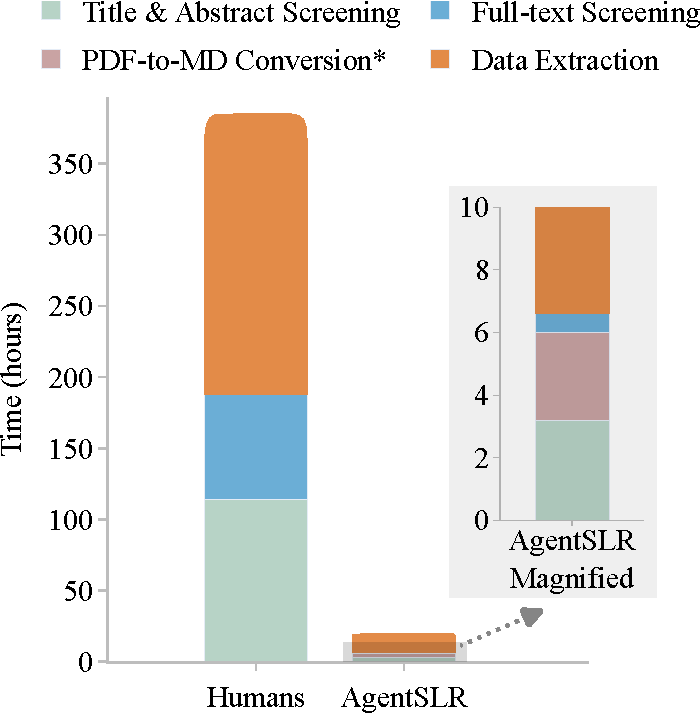
\includegraphics[width=0.375\textwidth]{figures/pipeline_stats/timeline_stats_vertical.pdf}
\caption{\textbf{Human vs. \name{} SLR completion time.} \name{} (with  \texttt{GPT-OSS-120B}) completes the end-to-end workflow in $20$ hours versus $385$ hours taken for manual-conducted reviews ({$19.3\times$} speed-up). Running continuously, this corresponds to less than 1 day ($0.83$) versus $48.1$ human workdays (assuming 8-hour days), yielding {$58\times$} calendar-time savings. Of \name{}'s run-time: data extraction accounts for $13.4$ hours ($67\%$), title and abstract screening for $3.2$ hours ($16\%$), PDF-to-MD conversion for $2.8$ hours ($14\%$), and full-text screening under $1$ hour. Times shown reflect processing of $9,132$ articles at abstract screening, $1,102$ at full-text screening and $395$ at data extraction. Report generation ($\leq$ $5$ minutes per pathogen) has been omitted. For more information, see Appendix~\ref{app:pipeline_statistics}.} \label{fig:time_comparison}
    \label{fig:time_comparison}
\end{figure}

\subsection{Metrics}

\paragraph{Pipeline runtime.} We evaluated \name{} first in terms of time efficiency relative to human annotators (\Cref{sec:full_pipeline_statistics}). We recorded the total wall-clock time to complete the first five pipeline stages and compare this time to self-reported estimates by human experts per stage. The final stage -- producing a final SLR for peer review -- does not admit a reliable time estimate, as it includes deliberations over meta-analysis outside the scope of \name{}, so we omitted this stage from our comparison.

%------------------------------
\paragraph{Individual pipeline stage evaluations.} To assess pipeline quality, we validated against expert annotations on four priority pathogens: Ebola, Lassa, SARS and Zika. 
We designed stage-level evaluations for each of abstract screening, full-text screening and data extraction. To isolate stage-level performance from compounding errors, each evaluation used ground-truth inputs for all previous stages.

Each of the two article screening stages is framed as a binary classification task, so we considered classification metrics (precision, recall, and $F_1$) against ground-truth screening decisions. Because the screening task is highly imbalanced, with far more excluded than included articles, we report these metrics and prioritise recall: false inclusions are easier to rectify at later pipeline stages, whereas missing articles cannot be corrected. For data extraction, quantifying agreement with ground-truth annotations is less straightforward. Each article may contain arbitrarily many extractions, and individual extractions may differ across many metadata fields. For a holistic account of \name's performance, we designed three evaluation measures. \textit{Flagging} assesses how reliably our pipeline identifies relevant parameter classes, models and outbreaks within an article. \textit{Count} measures agreement in the number of extracted items per article. \textit{Extraction} measures field-level accuracy by computing bipartite matches between our extractions and ground-truth extractions that maximise overall similarity. \Cref{app:additional_evaluation_details} provides formal definitions of the evaluation metrics and outlines pre-processing steps.
%------------------------------


\begin{figure*}[t!]
    \centering
    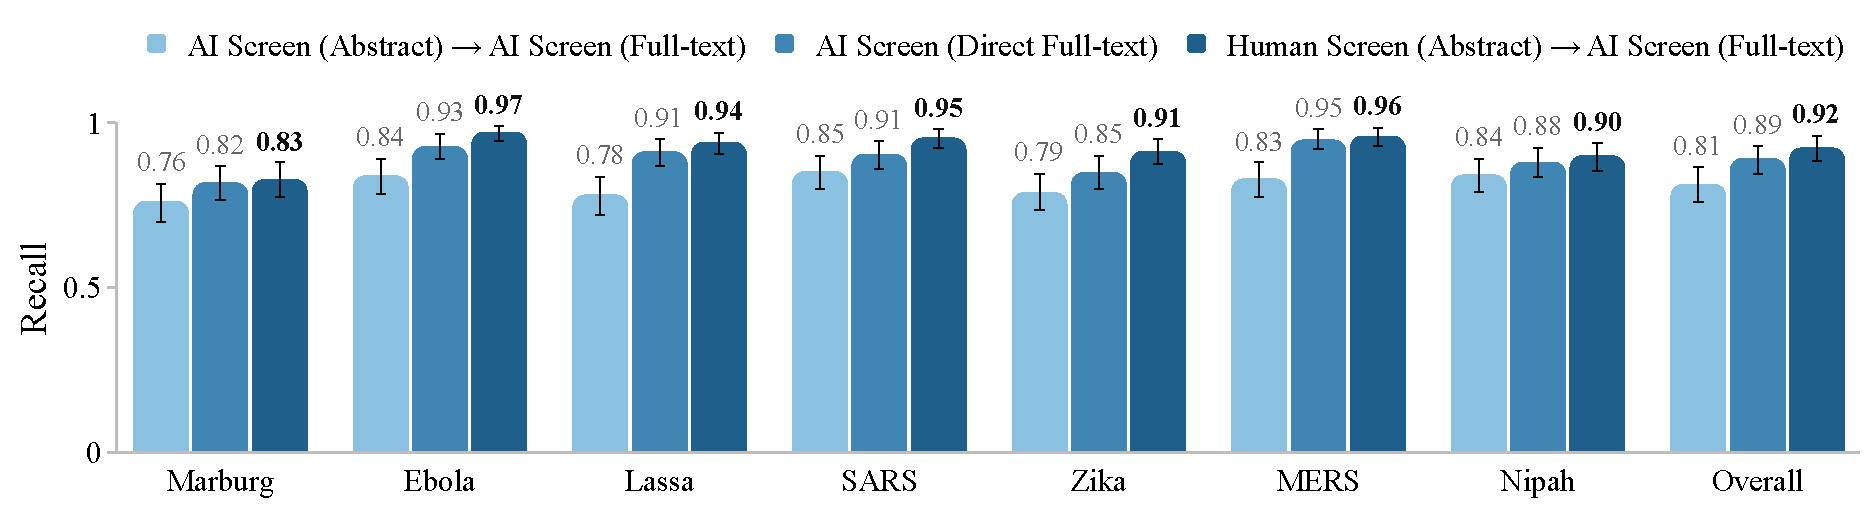
\includegraphics[width=1\linewidth]{figures/results/article_screening_recall.pdf}
    \caption{\textbf{Recall of article screening strategies across pathogens.} Two ablation screening strategies (human-conditioned, direct full-text) with \name{} (\texttt{GPT-OSS-120B}) offer better recall (or `fetch rate') than performing traditional AI-based two stage screening, with bootstrapped confidence intervals (95\% C.I.; 10{,}000 resamples) between the two ablations overlapping across most pathogens. Full article screening metrics along with individual title \& abstract stage screening results are reported in \Cref{app:extended_results_article_screening}.}
    \label{fig:fulltext_recall_barchart}
\end{figure*}

\paragraph{Human expert validation.}\label{sec:human_expert_validation_methods} Ground-truth screening decisions and annotations provide clear standards for recall---they allow us to check whether \name{} retrieves all relevant data. However, with respect to precision, it is ambiguous whether additional extractions represent genuine false positives or were instead missed by human annotators due to cognitive bandwidth constraints.

To supplement our individual stage evaluations, we conducted an additional validation with six expert epidemiologists. Each expert was assigned a random subset of extracted data for parameters, models or outbreaks, along with the corresponding markdown articles, and asked to grade extraction correctness using a survey. Survey questions included a yes/no question on the overall relevance of the extraction, yes/no questions for individual field correctness, and a holistic rating of \name{}'s capability for the task. For field-level correctness, we grouped fields by category (e.g. temporal features or population context) and reported normalised accuracy to assign equal importance to each group. Overall system capability was measured through ratings ranging between $1$ and $7$, where $1$ means total incompetence at the task, $4$ is the threshold for a useful tool under human supervision, and $7$ means completely competent and autonomous. System capability was rated for each extraction, providing a distribution of scores. \Cref{app:human_expert_validation} describes the survey design and implementation.


